\chapter{Random Variables}

\begin{ex}
  Note that
  \begin{align*}
    F(x^+)-F(x^-)
     & =F(x)-\lim_{\substack{y\to x    \\ y < x}}F(y) & & \text{(by Theorem 2.8)} \\
     & =\lim_{\substack{y\to x         \\ y < x}}F(x)-F(y) \\
     & =\lim_{\substack{y\to x         \\ y < x}}\P{X\leq x}-\P{X\leq y} \\
     & =\lim_{\substack{y\to x         \\ y < x}}\P{X\in (-\infty, x]}-\P{X\in (-\infty, y]} \\
     & =\lim_{\substack{y\to x         \\ y < x}}\P{X\in (-\infty, y]\cup(y, x]}-\P{X\in (-\infty, y]} \\
     & =\lim_{\substack{y\to x         \\ y < x}}\P{X\in (y, x]} \\
     & =\P{\bigcap_{i=1}^n (x-1/n, x]} \\
     & =\P{X=x}.
  \end{align*}
\end{ex}

\begin{ex}~
  \inputminted{python}{../code/02-02.py}

  \begin{figure}[H]
    \centering
    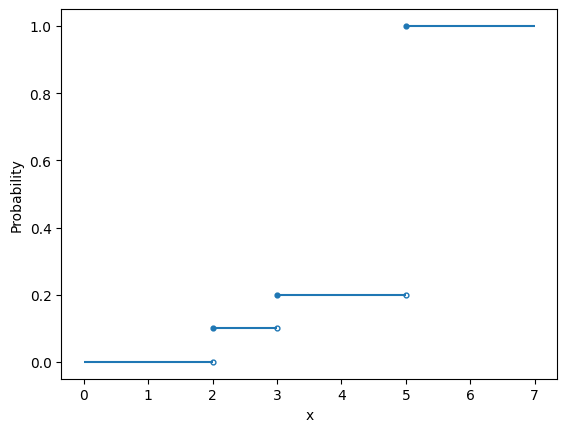
\includegraphics[scale=0.98]{../images/02-02}
    \caption{Plot of the CDF $F$.}
  \end{figure}

  Note that
  \[
    \P{2< X\leq 4.8}
    =\P{X\leq 4.8}-\P{X\leq 2}
    =\frac{2}{10}-\frac{1}{10}
    =\frac{1}{10},
  \]
  while
  \[
    \P{2\leq X\leq 4.8}=\P{X\leq 4.8}-\P{X< 2}=\frac{2}{10}-0=\frac{2}{10}.
  \]
\end{ex}

\begin{ex}
  \begin{enumerate}[1.]
    \item[]
    \item We already proved this claim as part of our solution to Exercise 1.
    \item Note that
          \begin{align*}
            F(y) - F(x)
             & = \P{X\in (-\infty, y]} - \P{X\in (-\infty, x]}           \\
             & = \P{X\in (-\infty, x]\cup(x, y]} - \P{X\in (-\infty, x]} \\
             & = \P{X\in (x, y]}                                         \\
             & = \P{x < X\leq y}.
          \end{align*}
    \item We have
          \begin{align*}
            \P{X>x}
             & = \P{X\in (x, \infty)}      \\
             & = \P{X\in (-\infty, x]^c}   \\
             & = 1 - \P{X\in (-\infty, x]} \\
             & = 1 - F(x).
          \end{align*}
    \item Note that by Part 2, $F(b)-F(a)=\P{a<X\leq b}$. Moreover, note that
          since $X$ is continuous, $\P{\{a\}}=\P{\{b\}}=0$, and hence we can
          freely add or remove the endpoints of the interval on the right-hand
          side without changing the value of the probability.
  \end{enumerate}
\end{ex}

\begin{ex}
  \begin{enumerate}[(a)]
    \item []
    \item We have
          \[
            F_X(x)=\begin{cases}
              0                                & x \leq 0,        \\
              \frac{1}{4}x                     & 0 < x < 1,       \\
              \frac{1}{4}                      & 1 \leq x \leq 3, \\
              \frac{1}{4} + \frac{3}{8}(x - 3) & 3 < x < 5,       \\
              1                                & x \geq 5.
            \end{cases}
          \]
    \item Let $Y=1/X$. Note that
          \[
            \P{Y\leq y}
            =\P{\frac{1}{X}\leq y}
            =\P{X\geq \frac{1}{y}}
            =1-F_X(y^{-1}),
          \]
          and that therefore
          \[
            F_Y(y)=\begin{cases}
              0                         & y\leq\frac{1}{5},          \\
              \frac{15}{8}-\frac{3}{8y} & \frac{1}{5}<y<\frac{1}{3}, \\
              \frac{3}{4}               & \frac{1}{3}\leq y\leq 1,   \\
              1 - \frac{1}{4y}          & y>1,
            \end{cases}
          \]
          and
          \[
            f_Y(y)=\begin{cases}
              0              & y\leq\frac{1}{5},          \\
              \frac{3}{8y^2} & \frac{1}{5}<y<\frac{1}{3}, \\
              0              & \frac{1}{3}\leq y\leq 1,   \\
              \frac{1}{4y^2} & y>1.
            \end{cases}
          \]
  \end{enumerate}
\end{ex}

\begin{ex}
  Let X and Y be independent discrete random variables. Then, for any
  $x,y\in\R$,
  \begin{align*}
    f_{X,Y}(x,y)
     & =\P{(X, Y)=(x, y)}            \\
     & =\P{(X, Y)\in \{(x, y)\}}     \\
     & =\P{X\in \{x\}, Y\in \{y\}}   \\
     & =\P{X\in \{x\}}\P{Y\in \{y\}} \\
     & =\P{X=x}\P{Y=y}               \\
     & =f_X(x)f_Y(y).
  \end{align*}

  Conversely, suppose that $f_{X,Y}(x,y)=f_X(x)f_Y(y)$ for all $x$ and $y$.
  Then for any $A$ and $B$,
  \begin{align*}
    \P{X\in A, Y\in B}
     & =\P{(X, Y)\in A\times B}                          \\
     & =\sum_{\substack{(a,b)\in A\times B}}f_{X,Y}(a,b) \\
     & =\sum_{a\in A}\sum_{b\in B}f_{X,Y}(a,b)           \\
     & =\sum_{a\in A}\sum_{b\in B}f_{X}(a)f_{Y}(b)       \\
     & =\sum_{a\in A}f_X(a)\sum_{b\in B}f_{Y}(b)         \\
     & =\P{X\in A}\P{Y\in B}.
  \end{align*}
\end{ex}

\begin{ex}
  Note that $Y$ is a discrete random variable with outcomes $0$ or $1$. In
  particular,
  \[
    \P{Y=1}=\E{I_A(X)}=\int_A\! f(x)\,\d{x},
  \]
  and therefore
  \[
    f_Y(x)=\begin{cases}
      1-\int_A\! f(t)\,\d{t} & x=0, \\
      \int_A\! f(t)\,\d{t}   & x=1.
    \end{cases}
  \]
  Hence,
  \[
    F_Y(x)=\begin{cases}
      0                      & x < 0,       \\
      1-\int_A\! f(t)\,\d{t} & 0\leq x < 1, \\
      1                      & x\geq 1.
    \end{cases}
  \]
\end{ex}

\begin{ex}
  Consider
  \begin{align*}
    \P{Z>z}
     & =\P{X>z}\P{Y>z}                                       \\
     & =(1-\P{X \leq z})(1-\P{Y \leq z})                     \\
     & =1-\P{X \leq z}-\P{Y \leq z}+\P{X \leq z}\P{Y \leq z} \\
     & =\begin{cases}
      1        & z< 0,       \\
      1-2z+z^2 & 0\leq z< 1, \\
      0        & z\geq 1,
    \end{cases}
  \end{align*}
  and hence
  \[
    f_Z(z)
    =\frac{\d}{\d{z}} F_Z(z)
    =\frac{\d}{\d{z}} (1 - \P{Z>z})
    =\begin{cases}
      2-2z & 0\leq z< 1,       \\
      0    & \text{otherwise}.
    \end{cases}
  \]
\end{ex}

\begin{ex}
  Note that $X^+$ is not supported on negative values and that therefore
  $\P{X^+\leq x}=0$ for $x<0$. Note that $X^+=0$ whenever $X\leq 0$ and
  therefore $\P{X^+=0}=\P{X<0}$. Finally, for $x>0$,
  \[
    \P{X^+\leq x}
    =\P{X^+<0}+\P{X^+=0}+\P{0<X\leq x}
    =F(0)+F(x)-F(0)=F(x).
  \]
  Hence,
  \[
    F_{X^+}(x)=\begin{cases}
      0    & x < 0,    \\
      F(x) & x \geq 0.
    \end{cases}
  \]
\end{ex}

\begin{ex}
  Suppose $X\sim \text{Exp}(\beta)$. Then
  \begin{align*}
    F(x)
     & =\int_{0}^x\!\beta e^{-\beta t}\,\d{t}                   \\
     & =-\int_{0}^{-\beta x}\!e^{u}\,\d{u}    &  & (u=-\beta t) \\
     & =1-e^{-\beta x}.
  \end{align*}
  Now, suppose that $q=1-e^{-\beta x}$. Then
  \[
    e^{-\beta x}= 1 - q,
  \]
  or,
  \[
    F^{-1}(q) = -\frac{\ln(1 - q)}{\beta}.
  \]
\end{ex}

% 10
\begin{ex}
  Let $A,B\subset \R$. Note that
  \begin{align*}
    \P{g(X)\in A, h(Y)\in B}
     & =\P{X\in g^{-1}(A), Y\in h^{-1}(B)}   \\
     & =\P{X\in g^{-1}(A)}\P{Y\in h^{-1}(B)} \\
     & =\P{g(X)\in A}\P{h(Y)\in B}.
  \end{align*}
  Since $A$ and $B$ were arbitrary, it follows that $g(X)$ and $h(Y)$ are
  independent.
\end{ex}

\begin{ex}
  \begin{enumerate}[(a)]
    \item[]
    \item Note that $\P{X=1}=\P{Y=1}=1/2$, but $\P{(X,Y)=(1,1)}=0$, instead of
          1/4 as we would have expected if $X$ and $Y$ were independent.
    \item We have
          \begin{align*}
            f_{N,X,Y}(n,x,y)
             & =f_{N}(n)f_{X|N}(x|n)f_{Y|X,N}(y|x,n)                                      \\
             & =\frac{\lambda^n e^{-\lambda}}{n!}\binom{n}{x}p^x(1-p)^{n-x}\delta(x+y-n),
          \end{align*}
          and therefore
          \begin{align*}
            f_{X,Y}(x,y)
             & =\sum_{n=0}^\infty\frac{\lambda^n e^{-\lambda}}{n!}\binom{n}{x}p^x(1-p)^{n-x}\delta(x+y-n) \\
             & =\frac{\lambda^{x+y} e^{-\lambda}}{(x+y)!}\binom{x+y}{x}p^x(1-p)^y                         \\
             & =e^{-\lambda}\frac{\lambda^x p^x}{x!} \frac{\lambda^y (1-p)^y}{y!}                         \\
             & =\frac{(\lambda p)^xe^{-\lambda p}}{x!} \frac{(\lambda(1-p))^ye^{-\lambda (1-p)}}{y!}      \\
             & = f_X(x)f_Y(y).
          \end{align*}
          Hence, by Problem 2.5, it follows that $X\amalg Y$.
  \end{enumerate}
\end{ex}

\begin{ex}
  Let $I_1\times I_2$ be the range of $X$ and $Y$ where $I_1$ and $I_2$ are
  (possibly unbounded) intervals. Then
  \begin{align*}
    f_X(x)
     & =\int_{I_2}\!f(x, y)\,\d{y}  \\
     & =\int_{I_2}\!g(x)h(y)\,\d{y} \\
     & =g(x)\int_{I_2}\!h(y)\,\d{y} \\
     & =h_0g(x),
  \end{align*}
  where the integral is known to be finite by Fubini's theorem since
  $\int_{I_1\times I_2}f(x,y)\,\d{(x,y)}=1$.

  Likewise,
  \[
    f_Y(y)
    =\int_{I_1}\!g(x)h(y)\,\d{y}
    =g_0h(y).
  \]

  Therefore,
  \[
    \int_{I_1}\!f_X(x)f_Y(y)\,\d{x}
    =h_0g_0\int_{I_1}\!g(x)h(y)\,\d{x}
    =h_0g_0\int_{I_1}\!f(x,y)\,\d{x},
  \]
  or, taking the leftmost and rightmost integrals,
  \[
    f_Y(y)=h_0g_0f_Y(y).
  \]
  Hence, $h_0g_0=1$, and so
  \[
    f_X(x)f_Y(y)=h_0g_0 g(x)h(y)=g(x)h(y)=f(x,y).
  \]
  Thus, $X$ and $Y$ are independent by Theorem 2.30.
\end{ex}

\begin{ex}
  \begin{itemize}[(a)]
    \item
          Note that
          \[
            F(y)
            =\P{Y\leq y}
            =\P{e^X \leq y}
            =\P{X \leq \ln {y}},
          \]
          and therefore
          \[
            f(y)
            =\frac{\d}{\d{y}}\Phi(\ln {y})
            =\frac{1}{y\sqrt{2\pi}}e^{-\frac{1}{2}(\ln{y})^2}.
          \]

          \inputminted{python}{../code/02-13a.py}
          \begin{figure}[H]
            \centering
            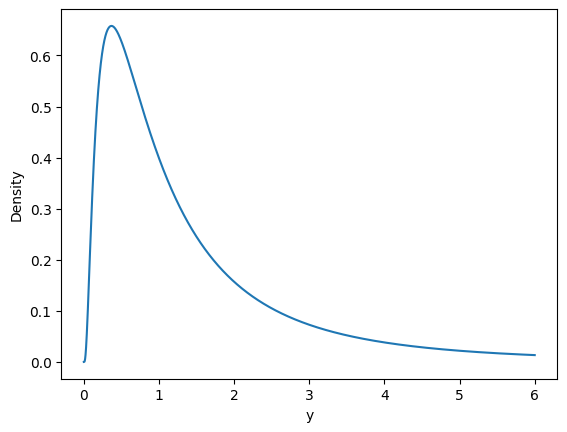
\includegraphics[scale=0.98]{../images/02-13a}
            \caption{Graph of PDF for $Y=e^X$.}
          \end{figure}

    \item[(b)]
          \inputminted{python}{../code/02-13b.py}

          \begin{figure}[H]
            \centering
            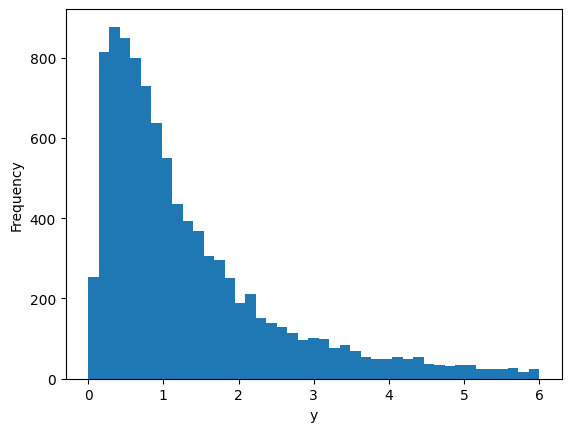
\includegraphics[scale=0.98]{../images/02-13b}
            \caption{Histogram of 10,000 samples from $Y=e^X$.}
          \end{figure}
  \end{itemize}
\end{ex}

\begin{ex}
  Note that since $(X,Y)$ is uniformly distributed, the probability that
  $\P{R\leq r}$ for $0\leq r<1$ is going to be proportional to the area of the
  disc of radius $r$. Therefore,
  \[
    F_R(r)=\begin{cases}
      0   & r < 0,          \\
      r^2 & 0\leq r \leq 1, \\
      1   & r > 1,
    \end{cases}
  \]
  and
  \[
    f_R(r)=\begin{cases}
      2r & 0\leq r \leq 1,   \\
      0  & \text{otherwise}.
    \end{cases}
  \]
\end{ex}

% 15
\begin{ex}
  We have
  \[
    F_X(x)
    =\P{X\leq x}         \\
    =\P{F^{-1}(U)\leq x} \\
    =\P{U\leq F(x)}
    =F(x),
  \]
  and therefore $X\sim F$.

  \inputminted{python}{../code/02-15.py}

  \begin{figure}[H]
    \centering
    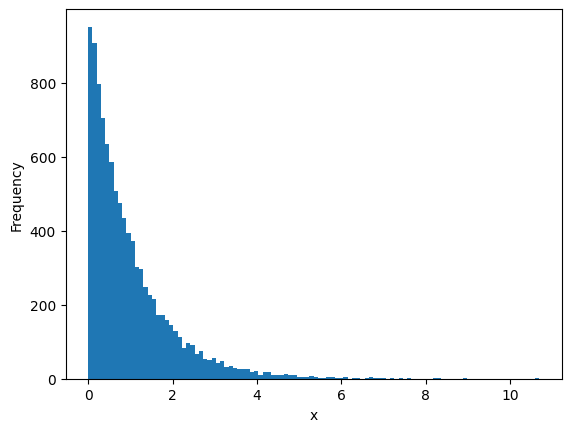
\includegraphics[scale=1]{../images/02-15}
    \caption{A histogram of samples drawn from a uniform distribution and then
      transformed under the inverse of the CDF of an $\text{Exponential}(1)$
      distribution.}
  \end{figure}
\end{ex}

\begin{ex}
  We have
  \begin{align*}
    \cP{X=x}{X+Y=n}
     & =\frac{\P{X=x,X+Y=n}}{\P{X+Y=n}}                                                                               \\
     & =\frac{\P{X=x,Y=n-x}}{\P{X+Y=n}}                                                                               \\
     & =\frac{\P{X=x}\P{Y=n-x}}{\P{X+Y=n}}                                                                            \\
     & =\frac{\lambda^x e^{-\lambda}}{x!}\frac{\mu^{n-x} e^{-\mu}}{(n-x)!}\frac{n!}{(\lambda +\mu)^ne^{-\lambda-\mu}} \\
     & =\binom{n}{x}\left(\frac{\lambda}{\lambda+\mu}\right)^x\left(\frac{\mu}{\lambda+\mu} \right)^{n-x}             \\
     & =\binom{n}{x}\left(\frac{\lambda}{\lambda+\mu}\right)^x\left(1-\frac{\lambda}{\lambda+\mu} \right)^{n-x},
  \end{align*}
  but this is precisely the probability mass function of a
  $\text{Binomial}(n, \lambda/(\lambda+\mu))$.
\end{ex}

\begin{ex}
  We begin by obtaining the marginal distribution for $Y$:
  \[
    \int_0^1\! c(x+y^2)\,\d{x}
    =c\left[\frac{x^2}{2}+xy^2\right]_{x=0}^1
    =c\left(\frac{1}{2}+y^2\right),
  \]
  and therefore
  \[
    f_Y(y)=c\left(\frac{1}{2}+y^2\right)I_{[0,1]}(y).
  \]

  Using the definition of conditional probability, we get
  \[
    f_{X|Y}(x\,|\,y)
    =\frac{f_{X,Y}(x,y)}{f_Y(y)}
    =\frac{(x+y^2)}{\left(\frac{1}{2}+y^2\right)}I_{[0,1]^2}(x,y).
  \]
  Therefore,
  \[
    \cP{X<\frac{1}{2}}{Y=\frac{1}{2}}
    =\int_0^{1/2}\!\frac{x+\frac{1}{4}}{\frac{1}{2}+\frac{1}{4}}\,\d{x}
    =\frac{4}{3}\int_0^{1/2}\!\left(x+\frac{1}{4}\right)\,\d{x}
    =\frac{1}{3}.
  \]
\end{ex}

\begin{ex}
  \begin{enumerate}[(a)]
    \item[]
    \item
          \begin{align*}
            \P{X<7}
            =\P{Z<\frac{7 - 3}{4}}
            =\P{Z<1}
            \approx 0.8413.
          \end{align*}
    \item
          \begin{align*}
            \P{X>-2}
            =1-\P{Z<\frac{-2 - 3}{4}}
            =1 - \P{Z<-1.25}
            \approx 0.8944.
          \end{align*}
    \item
          \begin{align*}
            .05
            =\P{X>x}
            =1-\P{Z<\frac{x-3}{4}}
          \end{align*}
          Therefore
          \begin{align*}
            1.64485\approx \Phi^{-1}(0.95)=\frac{x-3}{4},
          \end{align*}
          and so
          \begin{align*}
            x\approx 9.5794.
          \end{align*}

    \item
          \begin{align*}
            \P{0\leq X < 4}
             & =\P{X<4}-\P{X < 0}          \\
             & =\P{Z < 0.25}-\P{Z < -0.75} \\
             & \approx 0.3702.
          \end{align*}
    \item
          \begin{align*}
            .05
             & =\P{|X|>|x|}                                 \\
             & =\P{X>x}+\P{X<-x}                            \\
             & =1-\P{X<x}+\P{X<-x}                          \\
             & =1-\P{Z<\frac{x-3}{4}}+\P{Z<\frac{-x-3}{4}}.
          \end{align*}

          We use the following Python code to learn that $x$ is
          approximately $9.61098387$.

          \inputminted{python}{../code/02-18.py}
  \end{enumerate}
\end{ex}

\begin{ex}
  Suppose that $r$ is strictly monotone increasing with an inverse $s=r^{-1}$.
  Let $X$ be a random variable and let $Y=r(X)$.
  Then, since the inverse of a strictly monotone increasing function is also
  strictly monotone increasing,
  \[
    A_y
    =\{x \mid r(x) \leq y \}
    =\{x \mid x \leq s(y) \},
  \]
  and hence
  \[
    F_Y(y) = F_X(s(y)).
  \]
  Thus, by the Chain Rule,
  \[
    f_Y(y)=\frac{\d}{\d{y}}F_X(s(y))=f_X(s(y))\frac{\d{s(y)}}{\d{y}}.
  \]

  Next, suppose that $r$ is strictly monotone decreasing. Then, since the
  inverse of a strictly monotone decreasing function is also
  strictly monotone decreasing,
  \[
    A_y
    =\{x \mid r(x) \leq y \}
    =\{x \mid x \geq s(y) \}
  \]
  and hence
  \[
    F_Y(y) = 1-F_X(s(y)),
  \]
  and
  \[
    f_Y(y)=\frac{\d}{\d{y}}\left(1-F_X(s(y))\right)=-f_X(s(y))\frac{\d{s(y)}}{\d{y}}.
  \]

  Finally, note that in the strictly monotone increasing case,
  $\frac{\d{s(y)}}{\d{y}}>0$, and therefore we can replace it with
  $\left|\frac{\d{s(y)}}{\d{y}}\right|$, while in the strictly monotone
  decreasing case $\frac{\d{s(y)}}{\d{y}}<0$, and therefore we can replace
  $-\frac{\d{s(y)}}{\d{y}}$ with $\left|\frac{\d{s(y)}}{\d{y}}\right|$.
  Hence, in both cases
  \[
    f_Y(y)=f_X(s(y))\left|\frac{\d{s(y)}}{\d{y}}\right|.
  \]
\end{ex}

\begin{ex}
  Let $Z=X-Y$ and note that if $0<z\leq 1$,
  \[
    A_z=\{(x,y)\mid x-y\leq z\}
  \]
  is the unit square minus the triangle with vertices $(z,0)$, $(1,1)$ and
  $(1,1-z)$, while if $-1<z\leq 0$, $A_z$ is the triangle with vertices
  $(0, -z)$, $(0, 1)$ and $(1+z,1)$. Hence,
  \[
    F_Z(z)=\begin{cases}
      0                   & z\leq -1,         \\
      \frac{(1+z)^2}{2}   & -1<z\leq 0,       \\
      1-\frac{(1-z)^2}{2} & 0<z\leq 1,        \\
      1                   & \text{otherwise},
    \end{cases}
  \]
  and
  \[
    f_Z(z)=\begin{cases}
      1+z & -1<z\leq 0,       \\
      1-z & 0<z\leq 1,        \\
      0   & \text{otherwise}.
    \end{cases}
  \]

  Next, let $U=X/Y$, and note that then
  \[
    A_u=\{(x,y)\mid x/y\leq u\}
  \]
  is the area in the unit square above the graph of the line $y=\frac{1}{u}x$.
  If $0<u\leq 1$, this is the triangle with vertices $(0,0)$, $(0, 1)$ and
  $(u, 1)$, while if $u>1$, this is the entire unit square except the triangle
  with vertices $(0, 0)$, $(1, 0)$ and $\left(1, \frac{1}{u}\right)$. Therefore,
  \[
    F_U(u)=\begin{cases}
      0              & u\leq 0,   \\
      \frac{u}{2}    & 0<u\leq 1, \\
      1-\frac{1}{2u} & u> 1,
    \end{cases}
  \]
  and
  \[
    f_U(u)=\begin{cases}
      \frac{1}{2}    & 0<u\leq 1,        \\
      \frac{1}{2u^2} & u>1,              \\
      0              & \text{otherwise}.
    \end{cases}
  \]
\end{ex}

\begin{ex}
  Note that
  \begin{align*}
    F_Y(y)
     & =\P{Y\leq y}                                                                                   \\
     & =\P{X_1\leq y, X_2\leq y, \cdots, X_n\leq y}                                                   \\
     & =\P{X_1\leq y}\P{X_2\leq y}\cdots\P{X_n\leq y} &  & \text{(independence of $X_i$'s)}           \\
     & =\P{X_1\leq y}^n                               &  & \text{(identical distribution of $X_i$'s)} \\
     & =(1-e^{-\beta y})^n,
  \end{align*}
  and therefore,
  \[
    f_Y(y)
    =\frac{\d}{\d{y}} (1-e^{-\beta y})^n
    =n\beta e^{-\beta y}(1-e^{-\beta y})^{n-1}.
  \]
\end{ex}